% sets default font to Arial
\renewcommand{\rmdefault}{phv} % Arial
\renewcommand{\sfdefault}{phv} % Arial\\

%font size, document type and paper size
\documentclass[11pt,a4paper]{article}

\title{CMEE MRes Main Research Project}
\date{25 Aug 2019}
\author{Katherine Bickerton}

\usepackage[left=2cm,right=2cm,top=2cm,bottom=2cm]{geometry} % set page margins
\usepackage{lineno} % select specific line spacing
\linespread{1.5}
\usepackage{booktabs} % table formatting
\usepackage{multirow} % multiple header rows
\usepackage{pgfplotstable} % generate tables
\usepackage{graphicx} % inserting graphics
\usepackage{float} % positioning images
\usepackage[export]{adjustbox}
\usepackage{subcaption} % allow multiple figures
\usepackage{titlesec} % generate title page
\titleformat*{\section}{\large\bfseries}
\titleformat*{\subsection}{\normalsize\bfseries}
\usepackage{amsmath} % equation formatting
\usepackage{amssymb} % symbols for equations
\usepackage[comma]{natbib} % generate biblography
\bibliographystyle{unsrtnat} % specific style of bibliography
\usepackage{listings}



\begin{document}
	
	\begin{titlepage}
		\centering
		\topskip2cm
		
\includegraphics[width = 7cm,left]{../Results/imperial_logo.png}
		{\Large
			\vskip2cm
			What drives spatial and temporal patterns within the residential range of two commercially important \textit{Carcharhinus} species, and can they be used to predict broad scale displacements?
		}    
		\vskip1cm	
		{\large Katherine Bickerton\\
		Submitted: August 2019}
		\vskip2cm	
		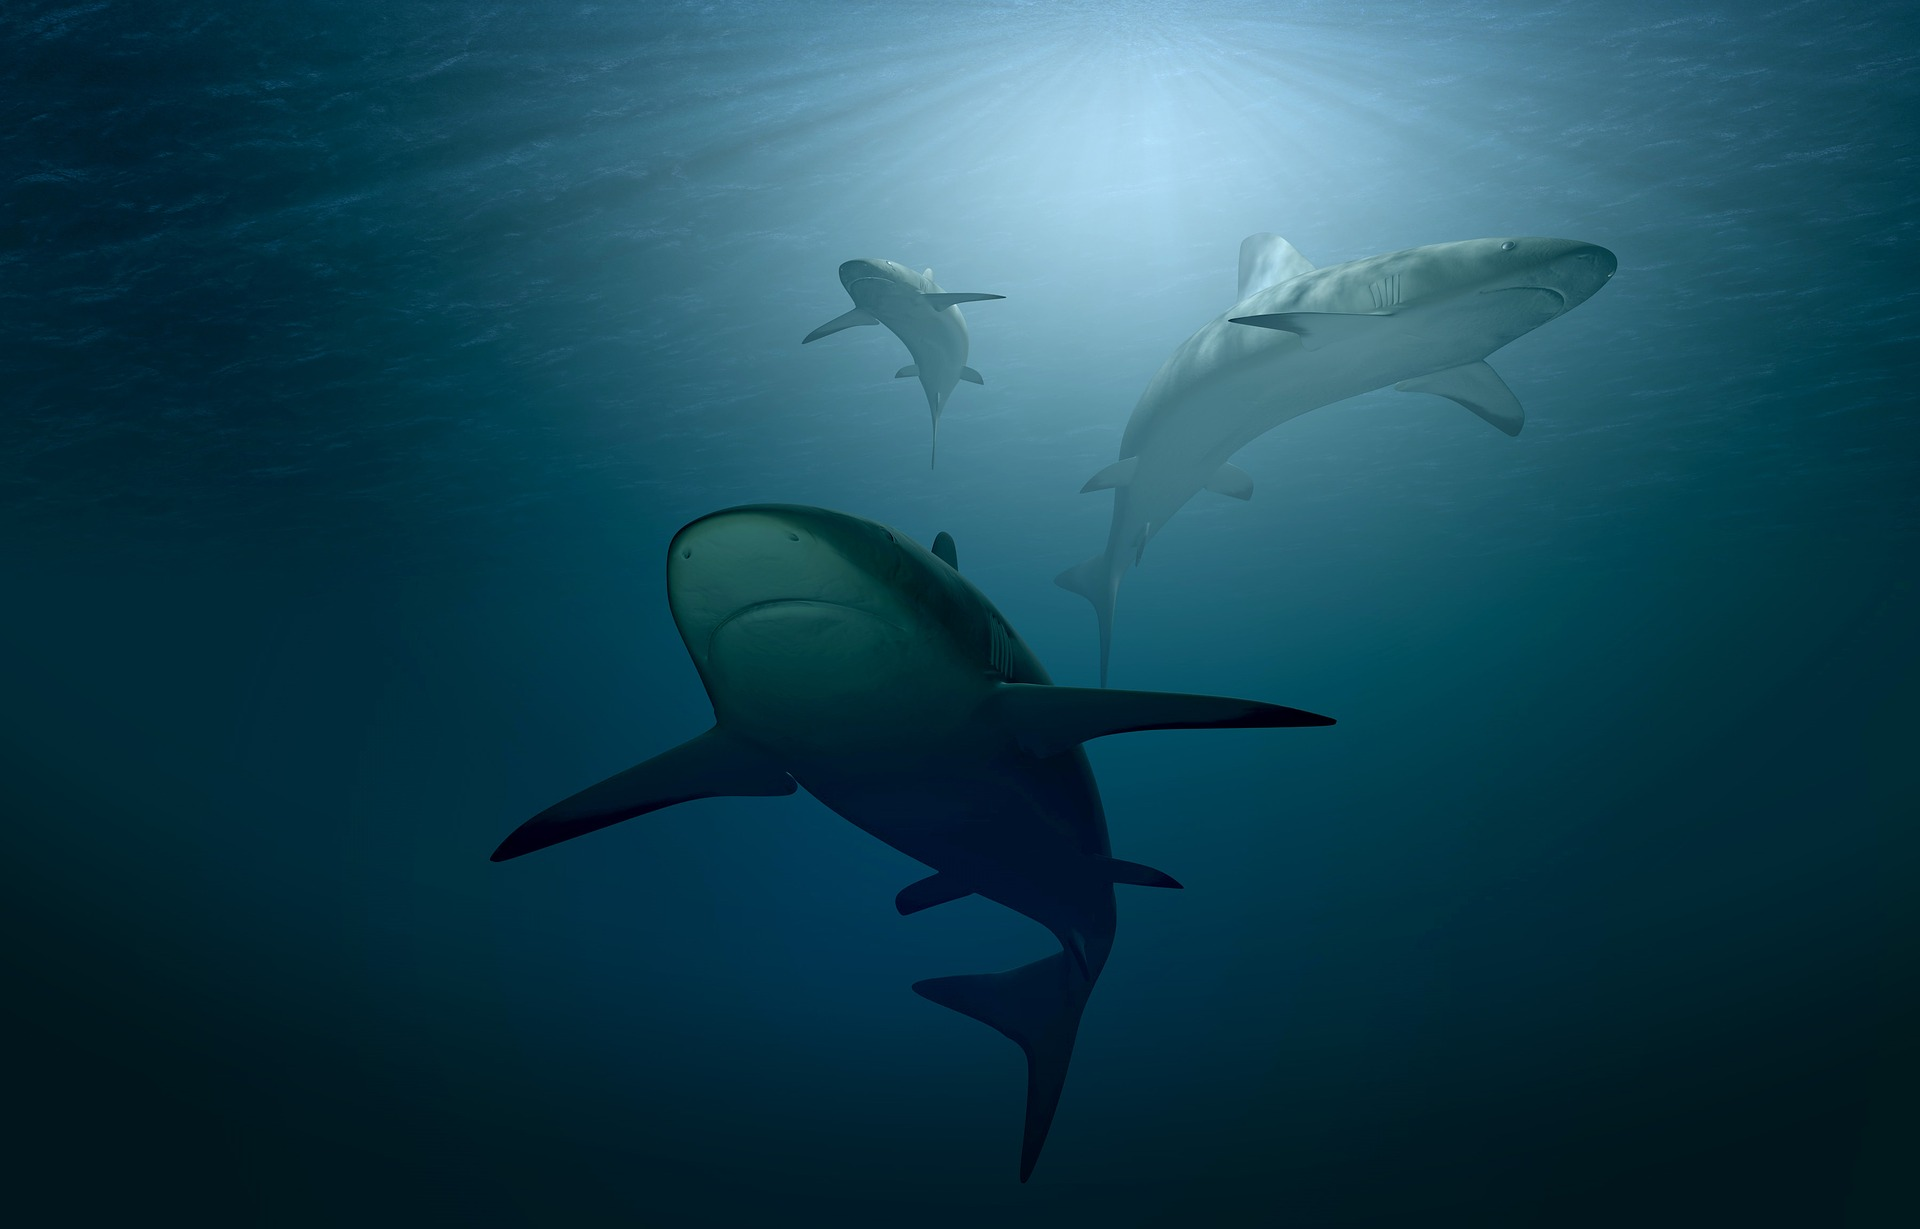
\includegraphics[width = 0.8\textwidth]{../Results/cover_image.jpg}
		\vskip3cm		
		\textbf{A thesis submitted in partial fulfilment of the requirements for the degree of Master of Research at Imperial College London\\
		Formatted in the journal style of the Marine Ecology Progress Series\\
		Submitted for the MRes in Computational Methods in Ecology and Evolution\\}
		\vspace*{\fill}
		\vspace*{\fill}
	\end{titlepage}
	
	
	\newpage
	
	\pagenumbering{gobble}
	\noindent{\large \textit{Declaration}}\\
	
	\noindent
	I declare that the data used in this project was collected and provided by my secondary supervisor Dr Matias Braccini, Western Australian Fisheries and Marine Laboratories, Government of Western Australia. I was provided with the raw dataset and carried out all processing, analysis and model development myself, with advice from Dr Matias Braccini and my primary supervisor, Dr David Jacoby, Institute of Zoology, Zoological Society of London. Dr Jacoby also provided training and R code for network analysis, which I adapted for the dataset used.
	
	
	
	\linenumbers
	\newpage
	\pagenumbering{arabic}
	
	\section{Abstract}
	
	
	\newpage
	
	\section{Introduction}
	
	The majority of sharks species are known to undertake large scale movements or regular migrations \citep{Speed2010,Espinoza2016}, on the scale of tens to thousands of kilometres \citep{Braccini2016a}. These movements enable connectivity between populations, and can prevent genetic drift and ultimately species persistence \citep{Olds2012,Espinoza2016}. However, broad scale marine movements are difficult to track, especially in highly mobile species such as sharks, which exhibit complex life histories \citep{Baeyaert2018}. This limits our understanding of the role that species play within ecosystems, their habitat use and threats facing them \citep{Espinoza2016}.\\
	\\
	A major threat to shark populations is overexploitation by commercial fisheries \citep{Worm2013}, both as targeted catch and as bycatch. Estimates of shark take ranged from 6.4 - 7.9\% of the global population \citep{Worm2013}, with high proportions of catches going unreported \citep{Clarke2006}. Shark finning is widely acknowledged as a driver of shark mortality due to the high value of fins in Eastern Asia \citep{Clarke2013}. Despite regulations against shark finning by countries including Australia, Brazil, the USA and the European Union \citep{Clarke2006,Benavides2011,Braccini2017c}, unregulated catches within Chinese waters and illegal catches globally, lead to high error margins in estimates of decline \citep{Worm2013}.\\
	\\
	Understanding movements is necessary for effective management and to mitigating against threats such as shark finning \citep{Espinoza2016}. One method of monitoring movements is the use of acoustic arrays and tags, which have traditionally be used over short spatial and temporal ranges \citep{Braccini2017}, however recent studies have used long term acoustic telemetry to determine fine scale movements in several species of reef shark \citep{Lea2016} and broader spatial scales in bull sharks, \textit{Carcharhinus leucas}, \citep{Espinoza2016}. Network analysis is also now regularly used in spatial studies, as it allows the interpretation of complex movement behaviours \citep{Lea2016}. Spatial network analyses allow the incorporation of biotic and abiotic factors, to build models and make predictions regarding future movements, making it a useful tool in conservation management \citep{Jacoby2016}.\\ 
	\\
	Movements of dusky, \textit{Carcharhinus obscurus}, and sandbar sharks, \textit{Carcharhinus plumbeus}, have been monitored using acoustic telemetry \citep{Braccini2016} and fisheries catch logs along the coast of Western Australia \citep{Braccini2017a}. Both species are of commercial importance to WA shark fisheries \citep{Braccini2017a} however both are also listed as Vulnerable by the IUCN Red List \citep{Musick2009,Musick2009a}, therefore understanding their movements is important economically and ecologically. As coastal species, they are at particularly high risk due to their close proximity to humans, leading to easier exploitation \citep{Espinoza2015} and a higher risk of habitat destruction \citep{Speed2010}. Additionally, both species have been previously overfished \citep{Benavides2011,Braccini2017a} and sandbar sharks have a particularly high fin to body size ratio making them more vulnerable to finning, due to higher fin value \citep{Braccini2017c}.\\
	\\
	Studies of \textit{C. obscurus} and \textit{C. plumbeus} have mainly examined large scale movements or movements of juveniles. The two species are often grouped as both are relatively long lived, late to mature and have long gestation periods \citep{Cortes2000,Benavides2011,Braccini2017c,Junge2019} adults are more important for population stability. There is evidence that mature \textit{C. obscurus} undertake periodic large scale migrations \citep{Hussey2009,Braccini2017b}, however there is little evidence of this in mature \textit{C. plumbeus} individuals \citep{Mcauley2005}. Furthermore, network analyses have not been applied to either species in WA and have yet to consider individual behaviours in addition to population trends.\\
	\\	
	This study will examine the movements of mature dusky and sandbar sharks within their residential range, Ningaloo Reef, WA, comparing the two species spatially and temporally. Network analyses will be applied to long term acoustic monitoring data, and individual scale behaviours examined. The aims of the study are to (1) compare variation in acoustic network use within and between species, (2) compare variation in area and depth use between and and within species and (3) compare residency patterns between and within species, all within their residential range with respect to individual, sex, season and time of day. This will then be linked as to what drives movements within the species home ranges and whether these movements can be extrapolated to give information regarding large scale movements.
	
	
	\newpage
	
	\section{Methods \& Materials}
	
	\subsection{Data Collection}
	
	In this study, acoustic telemetry was used to track the movements adult and sub-adult dusky sharks, \textit{Carcharhinus obscurus}, and sandbar sharks, \textit{Carcharhinus plumbeus}, over an array of 437 acoustic receivers located along the coast of Western Australia (Figure \ref{arrays}). Detection data was used from 2011 to 2018, with the first detection on the 2nd July 2011 and the last on the 5th September 2018. All shark tagging and deployment and retrieval of receivers was carried out by the Government of Western Australia’s Department of Fisheries (DoF), and raw dataset compiled by Dr Matias Braccini of the DoF.\\
	\\
	A total of 207 adult or sub-adult sharks, 103 \textit{C. obscurus} and 104 \textit{C. plumbeus}, were tagged between April and September 2011-2015 and 2017 by experienced taggers during surveys by the DoF. All sharks tagged were measured and sexed, and date and location of release recorded. Tagging was carried out along the coast between Broome and Esperance, WA, mainly within the Ningaloo reef (Figure \ref{releases}). For more details on the tagging procedure please refer to Braccini et al. \citeyear{Braccini2017c}.\\
	\\  
	The receivers were split into northern (Figure \ref{arrays}a) and southern arrays (Figure \ref{arrays}b \& c). In the north, 57 receivers were deployed in three lines arrays between the Tantabiddi Creek and Coral Bay, 21.5°S - 23.5°S, 113.5°E - 114°E, with a depth range of 2 – 161 meters. Although shark tagging occurred further to the north, cyclone exposure and the width of the continental shelf prevented more receivers from being deployed. The 380 southern receivers were split into five line arrays, two on the west coast and three on the south coast between Perth and the Recherche Archipelago, 31°S - 35.5°S, 114°E - 124°E, with a depth range of 9 – 198 meters. The receivers were initially set up to mitigate against white and tiger shark attacks in the south \citep{McAuley2016}, and to monitor coral reef fish spawning \citep{Babcock2017} therefore are in line arrays as opposed to the grids that are used in most network analysis experiments. For full details of the model of receivers used and data recovery, see \citealt{Braccini2017c,Braccini2017b}.\\
	\\
	During the eight years of monitoring, 130 of the 207 sharks tagged were detected (Table \ref{sum_stats}), 68 \textit{C. obscurus} and 62 \textit{C. plumbeus}, across 183 of the 437 receivers, with a total of 196,507 detections. The majority of these detections, 191,448, occurred with the residential range of both populations, the Ningaloo reef. Within the Ningaloo reef, 118 sharks were detected across 57 receivers. For each detection, the location, time, date, depth and tag code were recorded. This dataset, along with the size and sex data for each individual, and the location and depth of each receiver, was used in the analysis. \\
	
% Please add the following required packages to your document preamble:
% \usepackage{booktabs}
% \usepackage{multirow}
\begin{table}[h]
	\caption{Summary of detected shark demographics, where M, F and U stand for male, female and unknown respectively. Size range represents fork length, measured at time of tagging in meters. Time monitored is the number of days between tagging and the most recent detection.}
	\centering
	\begin{tabular}{@{}lcccccc@{}}
		\toprule
		\multirow{2}{*}{Species}       & \multicolumn{4}{c}{Sex} & \multirow{2}{*}{\begin{tabular}[c]{@{}c@{}}Size Range \\ (m)\end{tabular}} & \multirow{2}{*}{\begin{tabular}[c]{@{}c@{}}Time Monitored \\ (days)\end{tabular}} \\
		& M   & F   & U  & Total & & \\ 
		\midrule
		\textit{Carcharhinus obscurus} & 24  & 43  & 1  & 68 & 1.5 - 2.98 & 7 - 1987\\
		\textit{Carcharhinus plumbeus} & 19  & 43  & -  & 62 & 1.22 - 1.58  & 8 - 1976\\
		\midrule
		Total & 43  & 86  & 1  & 130    & - & - \\ 
		\bottomrule
	\end{tabular}
	\label{sum_stats}
\end{table}
	
\begin{figure}
	\centering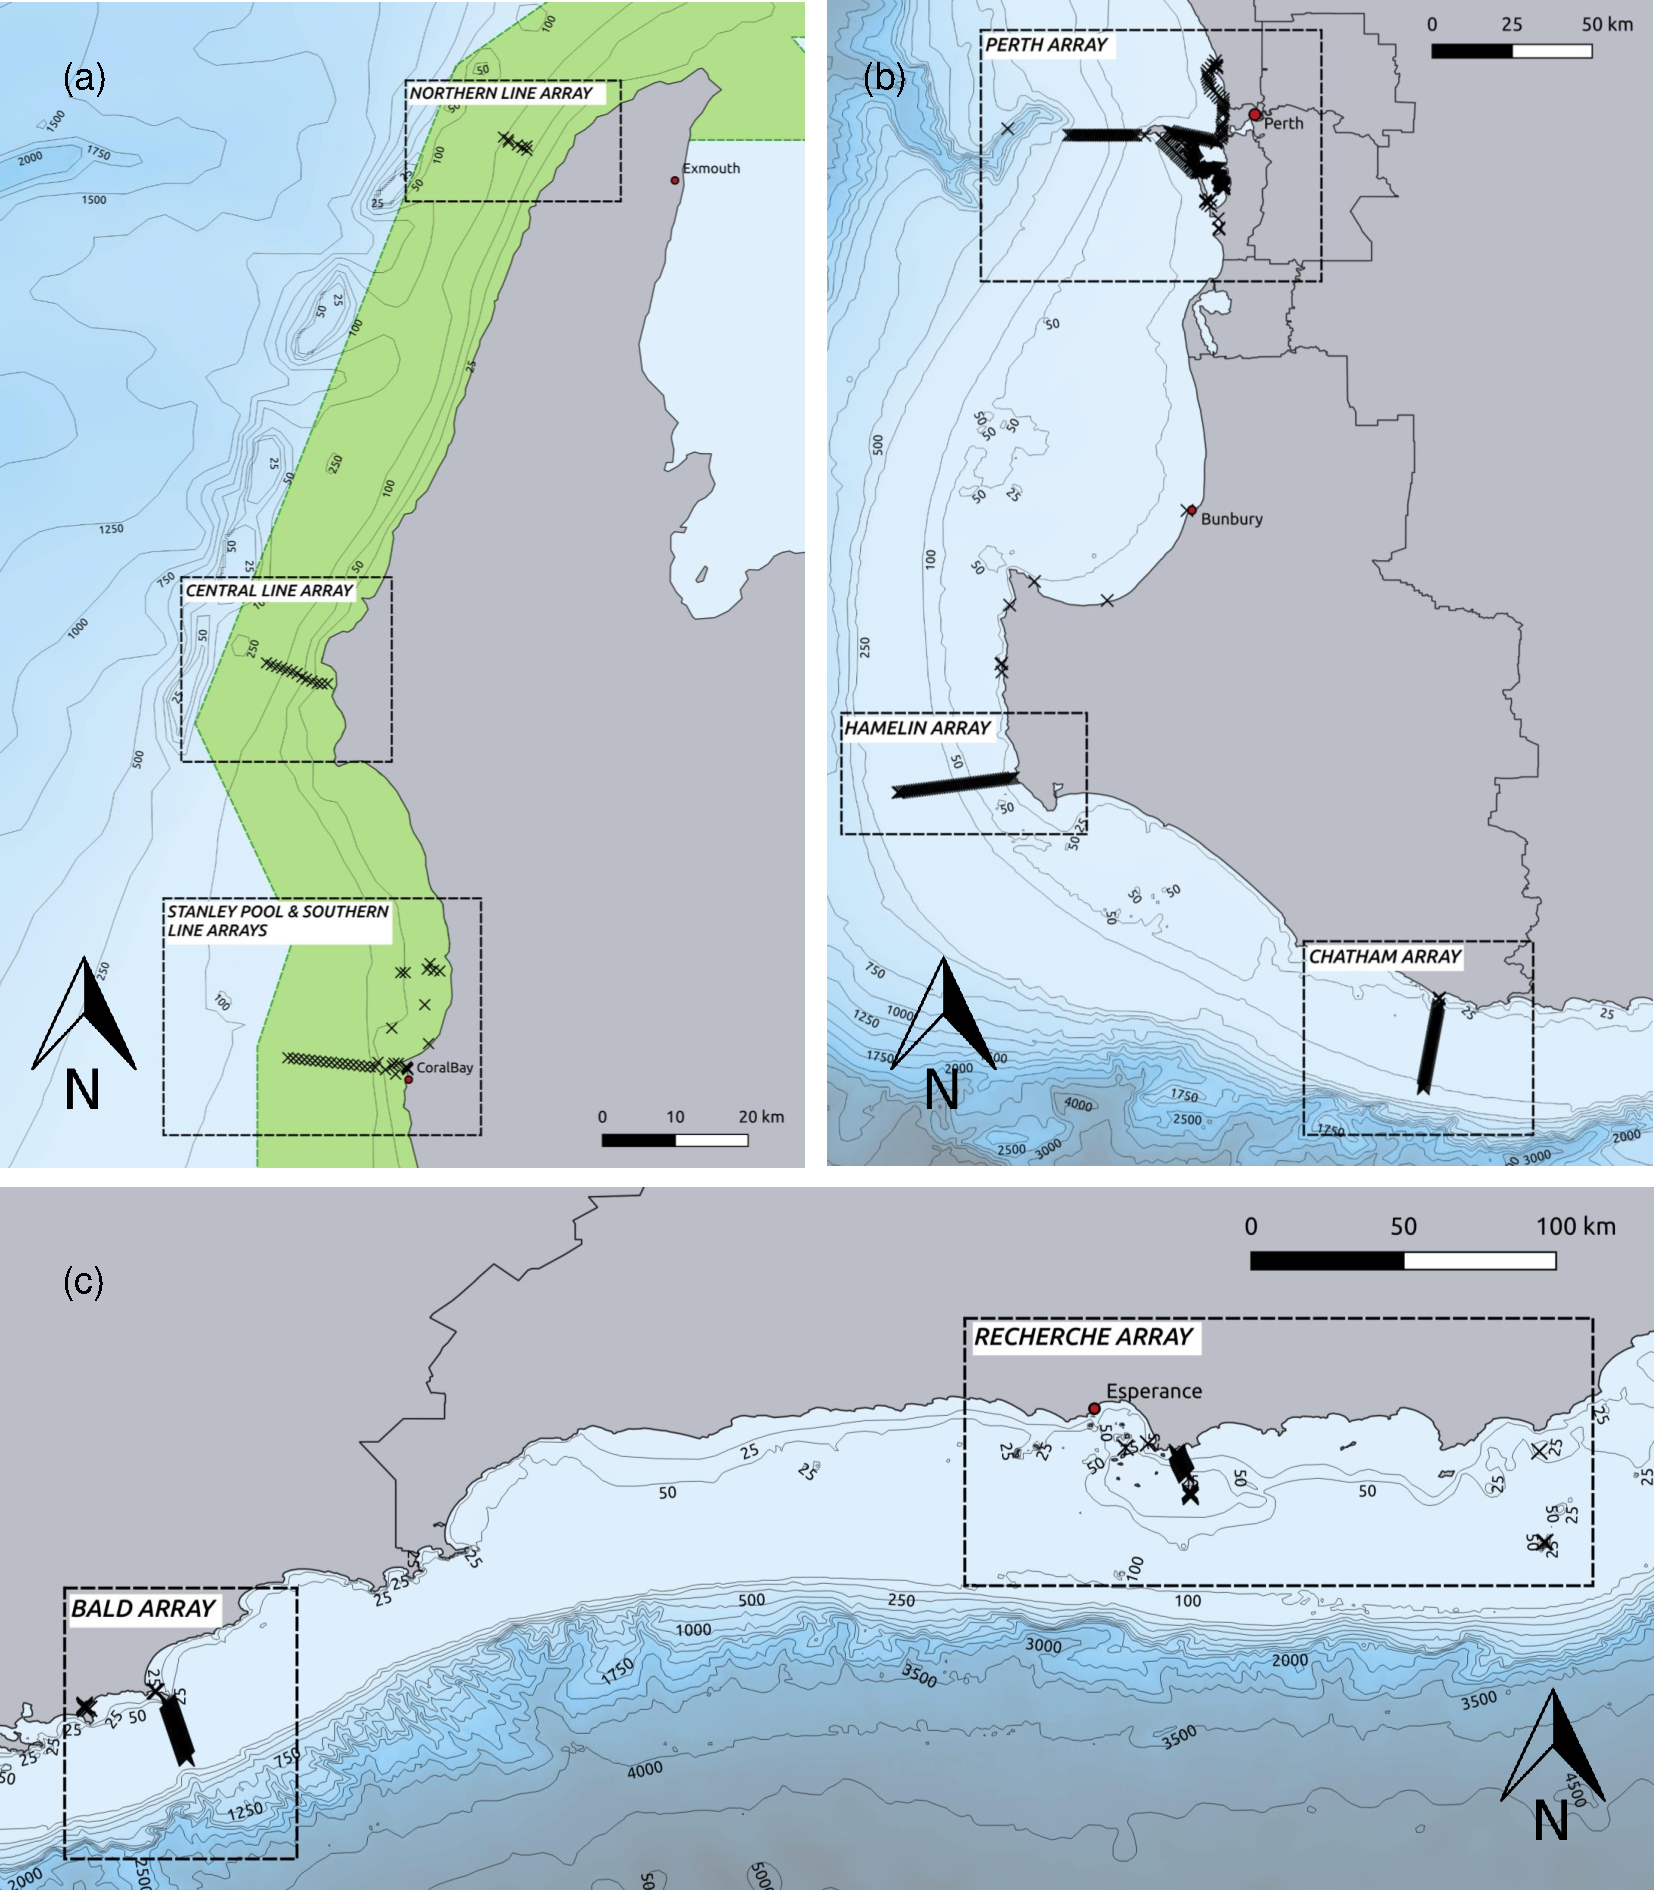
\includegraphics[width=\textwidth]{../Results/arrays_combined2.pdf}
	\caption{Distribution of acoustic receivers in Western Australia, each cross representing an individual receiver. (a) Northern receivers within the Ningaloo reef, total = 57, Northern Line array = 7, Central Line array = 13 and Stanley Pool and Southern Line arrays = 37. Green shading represents the Ningaloo marine World Heritage Site \citep{FlandersMarineInstitute2013}. (b) Perth and South Western receivers, total = 324, Perth array = 232, Hamelin array = 48 and Chatham array = 44. (c) Southern receivers, total = 56, Bald array = 33 and Recherche array = 23. This map was generated using QGIS \citep{QGISDevelopmentTeam2019}, with a base map shapefile \citep{AustralianBureauofStatistics2011}, bathymetric contour shapefile \citep{GEBCOCompilationGroup2019} and bathymetry raster \citep{Whiteway2009}.}
	\label{arrays}
\end{figure}

	

\begin{figure}
	\centering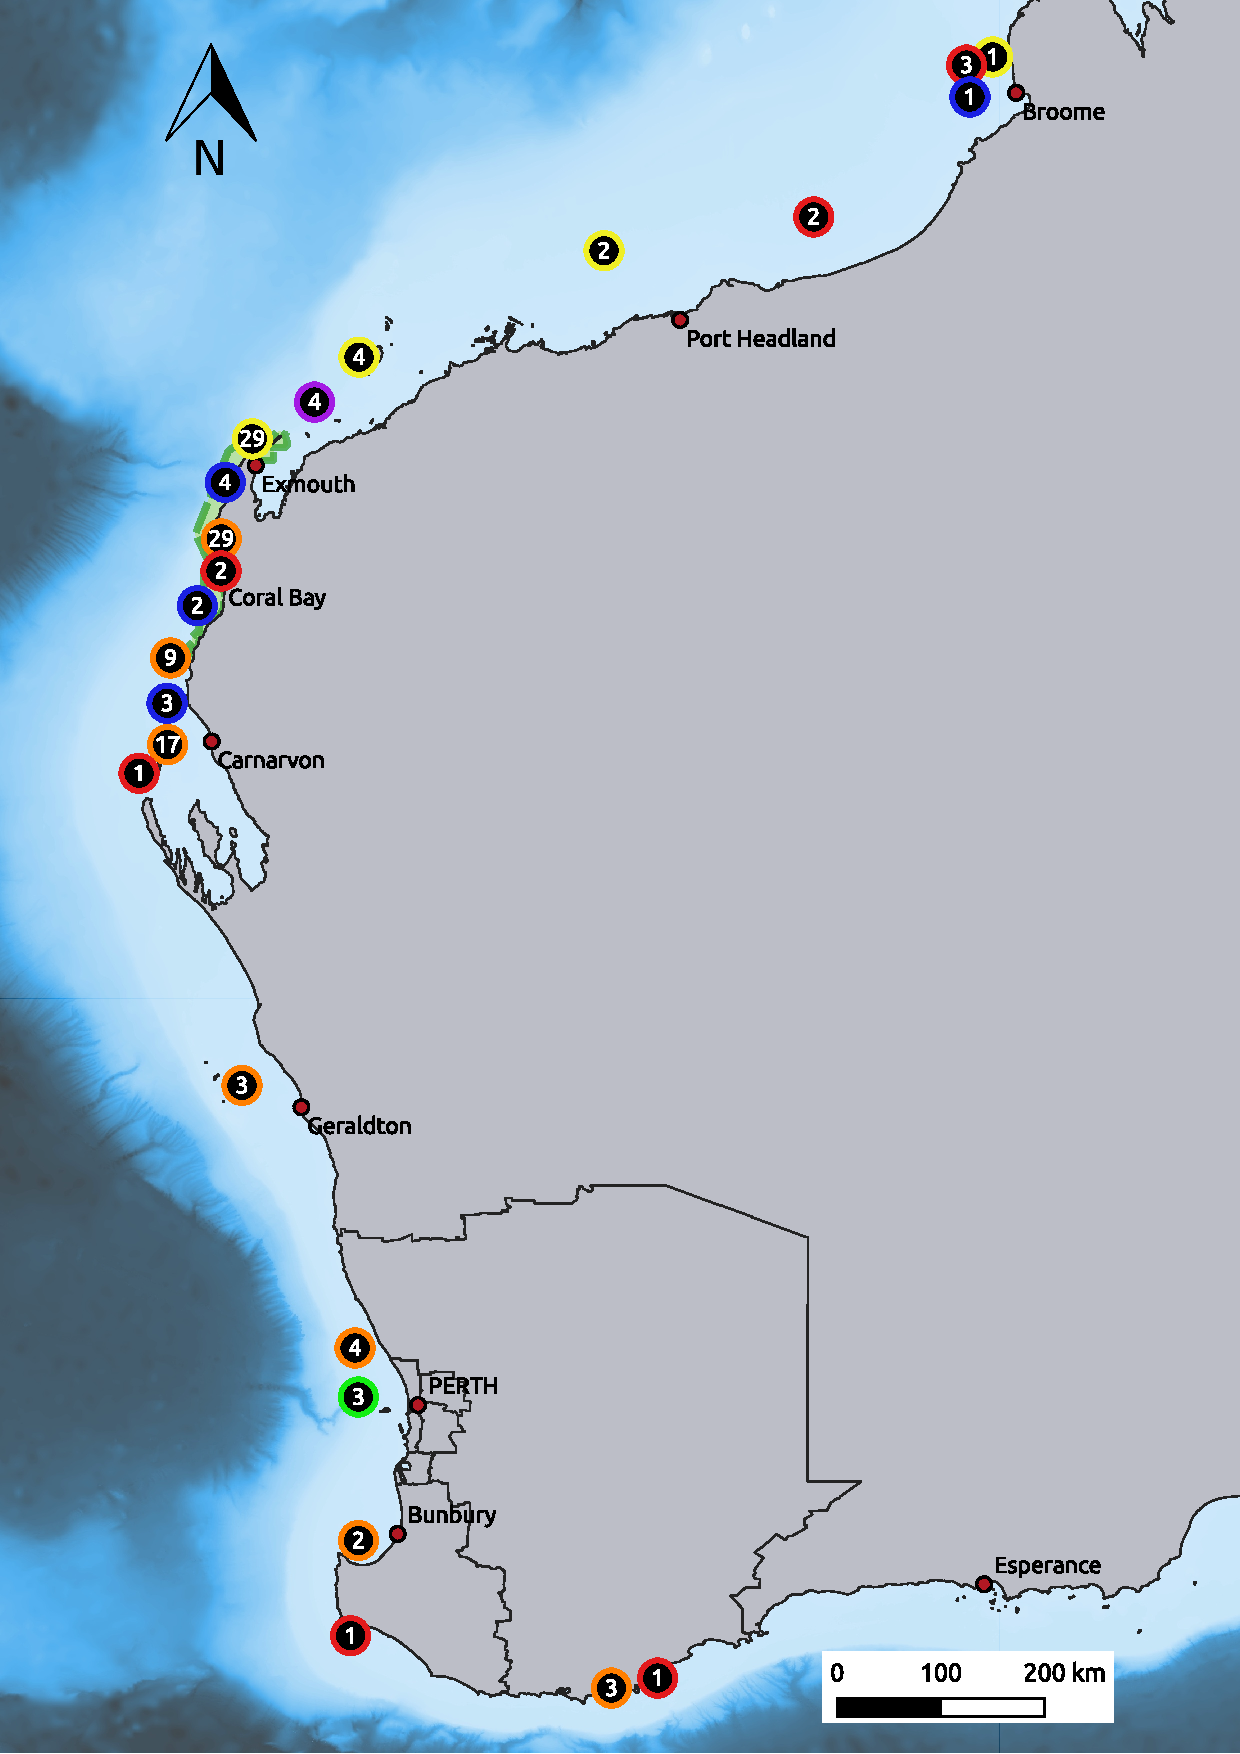
\includegraphics[width=0.6\textwidth]{../Results/Release_map.pdf}
	\caption{Locations of shark tagging of sharks detected between 2011 and 2018 (n = 130). The number within each circle gives the number of sharks tagged at that location and the coloured border gives the year of tagging (yellow = 2011, orange = 2012, red = 2013, purple = 2014, blue = 2015, green = 2017, no tagging occured in 2016 \& 2018.) This map was generated using QGIS \citep{QGISDevelopmentTeam2019}, with a base map shapefile \citep{AustralianBureauofStatistics2011} and bathymetry raster \citep{Whiteway2009}.}
	\label{releases}
\end{figure}

	
	\subsection{Data Analysis}
	
	All data manipulation, analysis and model building was carried out using R version 3.6.1 \citep{RCoreTeam2015}. The tidyverse package \citep{Wickham2017} was used for all data manipulation and plots and the lubridate package \citep{Grolemund2011} for formatting temporal data. Analyses used detections from the Ningaloo reef arrays exclusively (defined as any detection north of 24°S), as both species are show high residency to the reef \citep{Braccini2017}. The analysis was split into four sections: spatial network analysis, home range estimation using centres of activity, residency patterns using a residency index, and detection patterns examining detections per day. A combination of analyses methods were used as although spatial networks can be used to explain a movement dynamics, more traditional approaches can also provide valuable insight \citep{Baeyaert2018}. \\
	\\
	In each section of the analyses, linear mixed models were used to examine the relationship between the response variable (network density, kernel utilisation distribution, residency index and depth index respectively) and a range of fixed explanatory variables, using the lme4 R package \citep{Bates2015}. Linear mixed models were chosen so non-independent individual variation could be included as a random variable, and as data was linear but not normally distributed in all cases. Between and within species variation were both modelled. Model distribution was chosen by comparing the fit of quantile-quantile plots again normal, log normal, Poisson, negative binomial and gamma probability distributions, using the car \citep{Fox2019} and MASS \citep{Venables2002} packages in R. Test files were then generated, and each model tested, then outputs compared against the original data to check model fit, using the merTools package \citep{Knowles2019}.\\
	\\
	Fixed explanatory variables used were species, sex, season, time of day and migratory status. For sex, one individual of unknown sex was excluded. Season and time of day (day or night) were assigned based upon Austral seasons (Summer: December – February, Autumn: March – May, Winter: June – August, Spring: September – November) and average sunrise and sunset times per month across the years of monitoring \citep{GeoscienceAustralia2015}. Data was not stratified by year due to small sample sizes in several years. In models examining \textit{C. obscurus}, migratory status was used as an explanatory variable as the species are known to be resident in Ningaloo and make periodic migrations south \citep{Braccini2017b}. Migratory individuals were those that made at least one return journey between the Ningaloo receiver arrays and the southern arrays and were detected at least four times. Five \textit{C. obscurus} were only detected in the southern arrays and are shown to be younger individuals, most likely moving north from their nursery grounds, by \citealt{Braccini2017b}, so were also excluded from this study. Model selection was carried out using the Akaike Information Criterion (AIC), for each subset with best fit denoted by the lowest AIC value and highest marginal $R^2$ value, calculating using the MuMIn package for R \citep{Barton2019}, defined as individual variance explained \citep{Nakagawa2013}. Each model was then checked using a traditional likelihood ratio test (anova) comparing each model with a null model.\\
	
	
	\subsubsection{Spatial Networks}
	
	Network analysis examines the relationship between nodes and the connections between them, known as edges \citep{West2001}. In this system, the receivers are used as the nodes and individual shark movements as edges. Spatial networks were built for each species, sex and individual, then individual networks were subset by time of day and season. To generate each network, movements between receivers were calculated. The R package igraph \citep{Csardi2006} was used to calculate adjacency matrices and edge lists for each movement between receivers. Network density was calculated and is the number of edges in each network divided by the total number of possible edges \citep{Mourier2018}, representing the proportion of the total residential area (within the Ningaloo arrays) used by each individual. Network visualisations were generated using the rgdal package for R \citep{Bivand2019} to aid analysis. \\
	\\
	Network density was used as the response variable in each linear mixed model with a log normal probability distribution, and species, sex, season, time of day and migratory status (\textit{C. obscurus} only) as fixed explanatory variables. Any individuals with no movements detected were excluded. \\
	
	
	\subsubsection{Home Range}
	
	To investigate home range, centres of activity were calculated for each individual, and subset for each season and time of day. The centre of activity (COA) of each shark was calculated using the VTrack package \citep{Campbell2012}, which calculates a weighted mean position based upon detection locations. This method was evaluated and found to be reasonably accurate within an array when compared to actively tracked individuals \citep{Simpfendorfer2002}. The COAs were used to calculate minimum convex polygons (MCPs), which define the minimum area containing all detections of an individual, centred on the COA. To calculate these, a minimum of four detections at different receivers within the Ningaloo arrays were required, individuals that did not meet this criterion were excluded. MCPs give an estimate of the extent of range within the Ningaloo reef however a better estimate for home range is a kernel utilisation distribution (KUD). This method uses location and density of detections in a probability density function to estimate the probability of the individual being found within a certain area \citep{Jacoby2016}. Core or home range was then calculated as the area within the KUD where the most activity occurred, with a size of 50\% of the total KUD. MCPs and KUDs were calculated using the adehabitatHR package \citep{Calenge2006}, packages sp \citep{Pebesma2005,Bivand2013} and rgdal \citep{Bivand2019} were used to transform between coordinate systems and export shapefiles of KUD areas respectively. \\
	\\
	KUD area was used as the response variable for linear mixed models examining home range. The models used a gamma distribution, and species, sex, season, time of day and migratory status (\textit{C. obscurus} only) as fixed explanatory variables. Individuals with $<$5 movements in a subset were excluded, consistent with the overall COA calculations.\\
	
	
	\subsubsection{Residency Patterns}
	
	To study residency patterns within Ningaloo reef, a residency index was calculated for each individual over the monitoring period, and subsets taken and calculated for season, time of day and season stratified by time of day. The residency index was defined as the number of days detected within the Ningaloo arrays as a proportion of the number of days monitored, between release and last detection \citep{Espinoza2016}. Values near 1 indicate a high residency to the reef and 0 a low residency. \\
	\\
	Residency index was used as the response variable in the linear mixed models, with a log probability distribution (as the data was proportional). Fixed explanatory variables used were species, sex, season, time of day and migratory status (\textit{C. obscurus} only). Individuals detected on $<$5 unique days were excluded as sample size was too small to give an accurate measure of residency. \\
	
	
	\subsubsection{Detection Patterns}
	
	Number of detections per day per individual were calculated then split by depth to allow investigation of depth use. Depth of detections were split into 25m bands, with receiver depths ranging between 1 – 161 meters within Ningaloo reef. \\
	\\
	Mixed models were built using number of detections per day as response variable, with a log normal distribution. Fixed explanatory variables used were sex, species, depth band, time of day, season and migratory status (\textit{C. obscurus} only). To further examine depth patterns, fixed variables were tested as random variables with depth band as the only fixed variable, within further mixed models, again using a log normal distribution. Individuals with $<$5 unique days detected and depth bands with fewer than 5 detections were excluded in consistency with the rest of the study.\\
	
	
	\newpage
	
	\section{Results}
	
	To examine movement behaviour of dusky, \textit{Carchahinus obscurus}, and sandbar sharks, \textit{Carcharhinus plumbeus}, generalised linear mixed effect models (GLMMs) were used with spatial network density, kernel utilisation distribution area, residency index and detections per day as response variables. Within and between species variation was accounted for by modelling both species together and separately. Individual shark ID was used as a random effect to account for individual variation and non-independence of related individuals and all models used a single fixed explanatory variable. The best model for each response variable was selected using the Akaike Information Criterion (AIC), where the lowest value indicates best fit \citep{Bolker2009} and variance explained ($R^2$), where possible \citep{Nakagawa2013}. Traditional null model comparisons using likelihood ratio tests were also used as a third test of model fit however outputs from these were interpreted with caution as p-values are considered less relevant when using mixed effect models \citep{Posada2004}. Models with multiple explanatory variables were tested and found, in all cases, to explain less of the variance and have a higher AIC value than models with single variables. Full model outputs can be found in the Appendices. 
	
	
	\subsection{Spatial Networks}
	
	Network density was used as the response variable for all spatial network models and gives the proportion of edges in the network used out of all possible edges \citep{Mourier2018}. Individual variation accounted for between 65.5 - 91.2\% of deviance explained in each model, indicating high intra-species variation in network use. Detailed outputs of all models in this section are given in Appendix Table A1.\\
	\\	
	Species, as a fixed effect, had a relatively low AIC value (65.60) and accounted for 4.7\% of deviance, with sandbar sharks using a higher proportion of the network than dusky sharks, on average (Figure \ref{net_seasons}). Sex had the highest AIC (67.52) and explained 4.9\% of deviance across both species, with males using a slightly higher proportion of the network overall but not significantly so. Season gave the lowest value of AIC (65.09) and accounted for 3.2\% of deviance. Highest network density occurred in Summer then decreased through Autumn into Winter, then increased again in Spring (Figure \ref{net_seasons}). Network density did not vary significantly with time of day, accounting for only 1\% of deviance.\\
	\\
	When subset for \textit{C. obscurus}, sex accounted for 13\% of deviance, with males having a higher network density than females. Seasonal variation gave the lowest AIC value (48.39) and accounted for 15.9\% of deviance, with the same pattern as before, highest in summer, decreasing through autumn to winter then increasing again in spring (Figure \ref{net_seasons}). Time of day and migratory status accounted for 2.1\% and 3.4\% of deviance respectively and showed very little variation.\\
	\\
	Network density in \textit{C. plumbeus} again showed greatest variation and lowest AIC value (5.12) seasonally, which accounted for 3.3\% of deviance. The highest value of network density occurred in summer and decreased through to winter as before, however continued to decrease in spring (Figure \ref{net_seasons}). Time of day and sex showed minimal variance and gave significantly higher AIC values of 8.46 and 9.42 respectively.
	
	\begin{figure}[h]
		\centering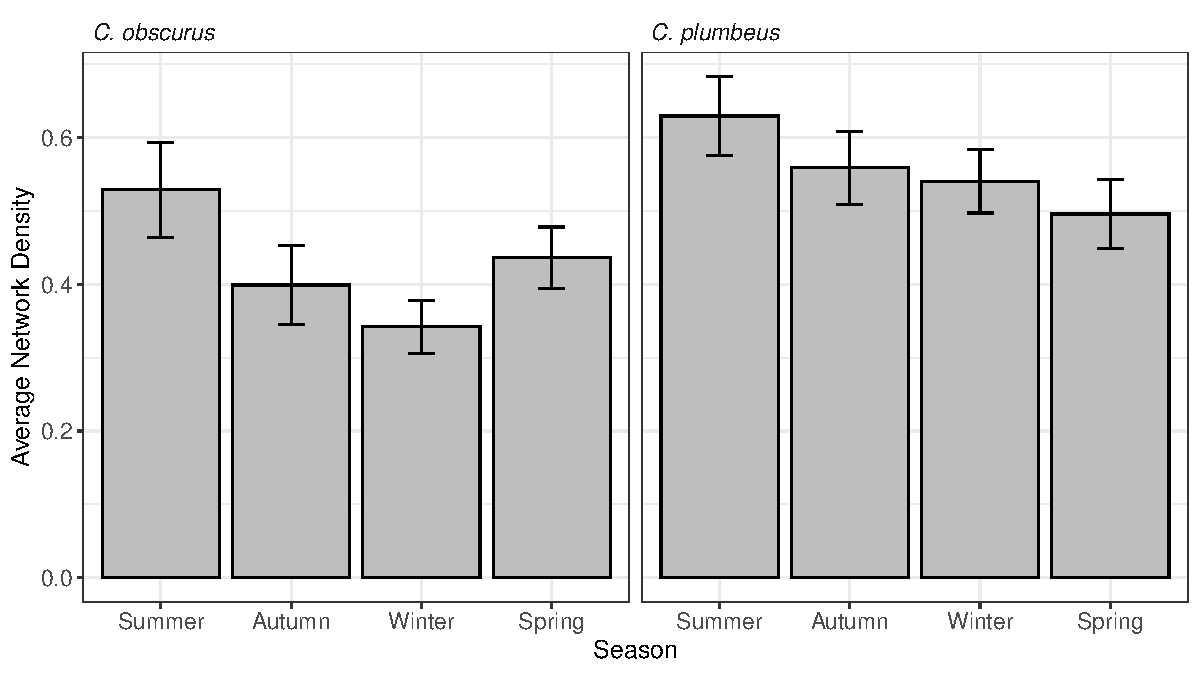
\includegraphics[width=\textwidth]{../Results/network_season.pdf}
		\caption{Seasonal variation in network density of \textit{Carcharhinus obscurus} (n = 53) and \textit{Carcharhinus plumbeus} (n = 58). Bars give mean average network density and error bars give standard error. Seasons are defined as standard Austral seasons.}
		\label{net_seasons}
	\end{figure}
	
			
	\subsection{Home Range}
	
	Kernel utilisation area (KUD) was used as the response variable in each home range model, and gives the size of the core range of each individual, based upon detection number and location \citep{Jacoby2016}. Model were selected using AIC and with reference to likelihood ratio tests as $R^2$ lack accuracy for gamma distributed models. Individual variation had a significant effect in all models when tested against a null linear model.\\  
	\\
	The largest variation in KUD was between species, with the lowest AIC values for both season and time of day subsets (334.9 and 285.8), and a significant difference with the null GLMM (ANOVA: $\chi^2_4$ = 12.13, \textit{p} \textless 0.001). \textit{C. obscurus} had a larger average kernel area than \textit{C. plumbeus}. Intraspecies variation in area was also much lower in \textit{C. plumbeus} than in \textit{C. obscurus}. KUD showed little variation with sex, season, time of day or migratory status in all subsets. All model outputs are given in Appendix Table A2. 
	
	
	
	%\begin{figure}[h!]
	%	\centering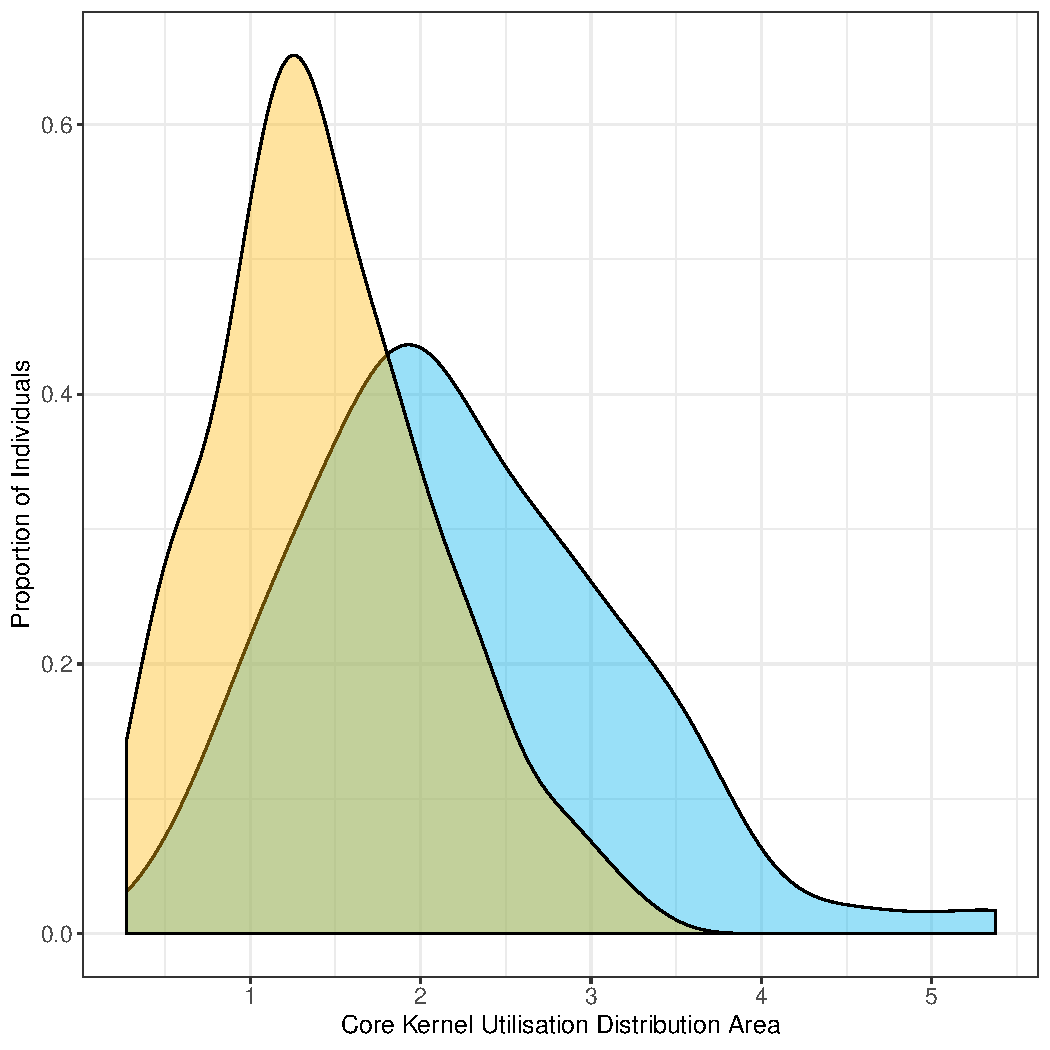
\includegraphics[width=0.65\textwidth]{../Results/KUD_densityplot_sp.pdf}
	%	\caption{Size of kernel utilisation area ($km^2$) as a proportion of each shark population. Blue = dusky (\textit{Carcharhinus obscurus}, n = 38) and yellow = sandbar sharks \textit{Carcharhinus plumbeus}, n = 39).}
%		\label{kud_species}
%	\end{figure}
	
	
	\subsection{Residency Patterns}
	
	Residency index (RI) was calculated as days detected within the Northern receiver arrays (Figure \ref{arrays}a), as a proportion of days monitored, and used as the response variable for all residency models. Individual variation was significant in all models, accounting for between 77.6 - 99.5\% of deviance explained by each model. Full model outputs are available in Appendix Table A3.\\
	\\
	There was little variation in RI with species and sex, and relatively high values of AIC (-345.8,-644.9), and low deviance explained (3.8\% and 1.8\%). RI varied with season, with the lowest AIC value of -710.7. RI decreased in summer and spring but was more consistent in autumn and winter, however this only explained 3.7\% of the deviance. Seasonally, average sandbar RI was higher than dusky (Figure \ref{ri_seasons}). Time of day also led to variance in RI, with residency being slightly higher at night, however only 0.6\% deviance was explained by this model.\\
	\\
	
	\begin{figure}[h!]
		\centering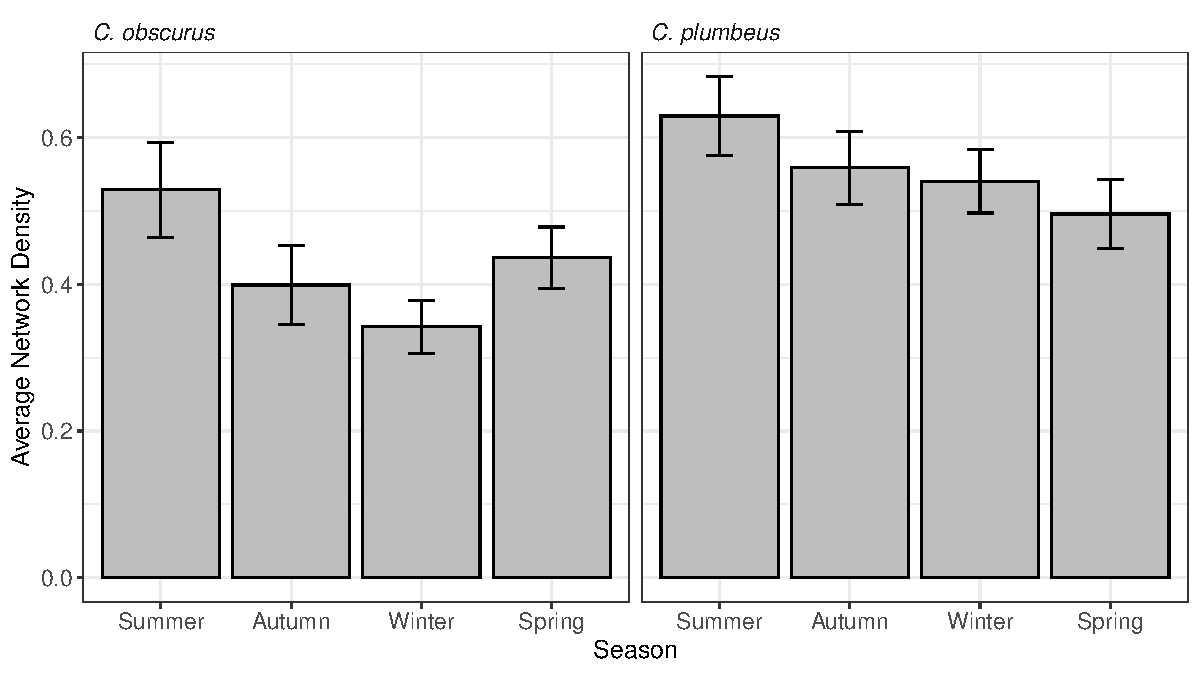
\includegraphics[width=0.9\textwidth]{../Results/network_season.pdf}
		\caption{Seasonal variation in residency index of \textit{Carcharhinus obscurus} (n = 51) and \textit{Carcharhinus plumbeus} (n = 59). Bars give mean average residency index and error bars give standard error. Seasons are defined as standard Austral seasons.}
		\label{ri_seasons}
	\end{figure}		
	
	\noindent RI varied more significantly by season within the \textit{C. obscurus} subset, explaining 22.2\% of deviance, and having the lowest AIC of -461.8. RI was lowest in the summer, then increased through autumn and winter, then decreased again in spring (Figure \ref{ri_seasons}). Time of day also had a low value of AIC within it's subset (-740.5), with a slight increase in RI at night but only this accounted for 5\% of deviance. Sex explained 18.2\% of deviance in RI, with higher RI in females, but a high AIC value. RI did not vary with migratory status. \\
	\\
	Seasonal variation was also present in the \textit{C. plumbeus} subset, with a AIC of -349, with values highest in summer, decreasing until Spring but only by a small proportion (Figure \ref{ri_seasons}). Time of day and sex had very little effect on RI for sandbars, with a slightly higher average RI at night and in males.
	
	

	\subsection{Detection Patterns}
	
	Number of detections per day was used to examine detection patterns and calculated for each individual, per depth band (set at 25m intervals). AIC were all exceptionally high and $R^2$ values very low for all models examined in comparison to all other response variables. Individual variation accounted for between 12.0 - 24.3\% of deviance in each model and all fixed effects accounted for \textless0.1\%. See Appendix Table A4 for all model outputs.\\
	\\
	Depth of detections, although have a low $R^2$ and high AIC value, did highlight seasonal trends. Detections of \textit{C. obscurus} between 0-25m and over 100m only occurred in winter and spring, whereas detections between 25-100m occurred in all seasons. None were detected above 125m. Detections of \textit{C. plumbeus} between 0-125m occurred during all seasons, however the number of detections at depths below 25m were significantly lower. \textit{C. plumbeus} were detected at depths \textgreater125m but only during winter and autumn. The northern lines array in Figure \ref{depth_north} shows the near constant distribution of sandbar sharks (orange) throughout the year and absence of dusky sharks (purple) in the summer. The central line array, Figure \ref{depth_mid}, shows the decrease in dusky sharks in summer and a more restricted depth range in the spring. The Stanley Pool and southern line arrays, Figure \ref{depth_south}, show a decrease in dusky sharks through spring and summer, as well as more shallow water detections than in sandbars. Figures \ref{depth_north}-\ref{depth_south} all highlight the greater depths at which sandbars are found throughout the year.
	
	
	\begin{figure}[h!]
		\centering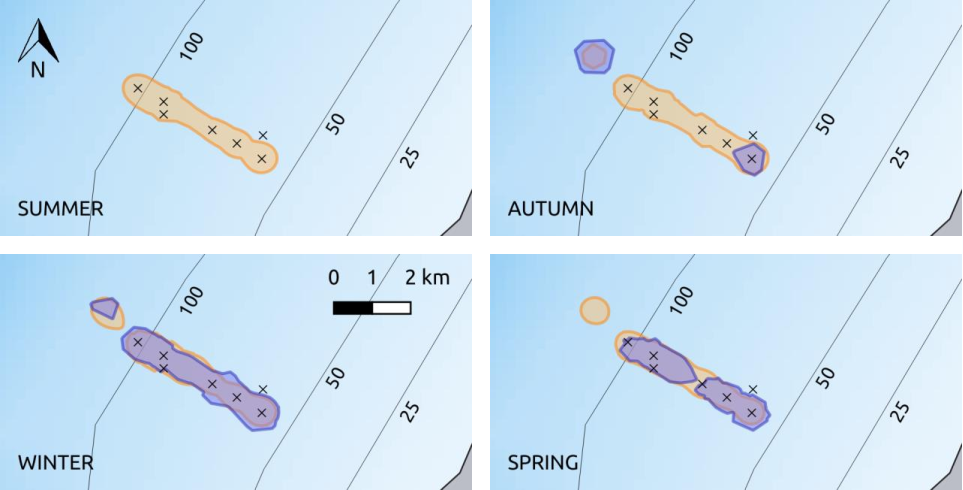
\includegraphics[width=0.85\textwidth]{../Results/north.pdf}
		\caption{Seasonal variation in core kernel utilisation areas of \textit{Carcharhinus obscurus} (purple) and \textit{Carcharhinus plumbeus} (orange), within the northern line array, Ningaloo reef, WA. Black crosses show acoustic receiver locations and water depth is given parallel to each bathymetry contour This map was generated using QGIS \citep{QGISDevelopmentTeam2019}, with a base map shapefile \citep{AustralianBureauofStatistics2011}, bathymetric contour shapefile \citep{GEBCOCompilationGroup2019} and bathymetry raster \citep{Whiteway2009}.}
		\label{depth_north}
	\end{figure}		
	\begin{figure}[h!]
		\centering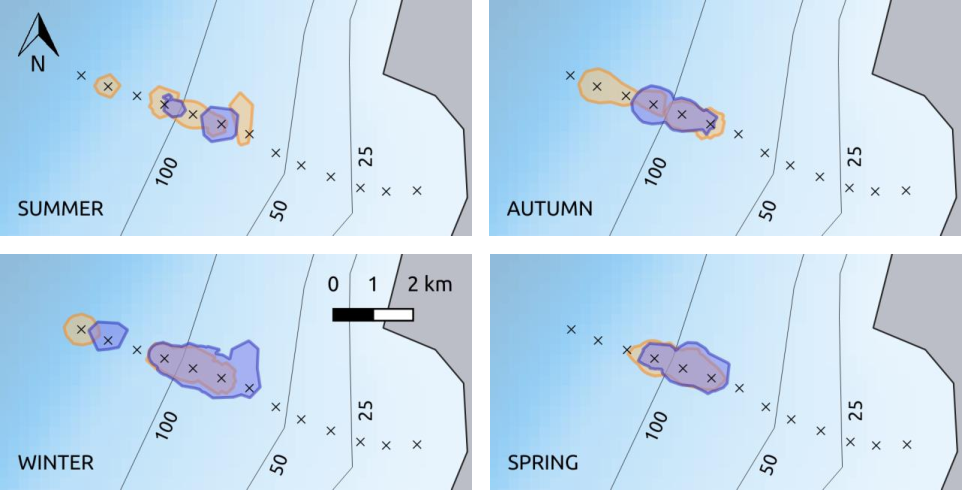
\includegraphics[width=0.85\textwidth]{../Results/mid.pdf}
		\caption{Seasonal variation in core kernel utilisation areas of \textit{Carcharhinus obscurus} (purple) and \textit{Carcharhinus plumbeus} (orange), within the central line array, Ningaloo reef, WA. Black crosses show acoustic receiver locations and water depth is given parallel to each bathymetry contour This map was generated using QGIS \citep{QGISDevelopmentTeam2019}, with a base map shapefile \citep{AustralianBureauofStatistics2011}, bathymetric contour shapefile \citep{GEBCOCompilationGroup2019} and bathymetry raster \citep{Whiteway2009}.}
		\label{depth_mid}
	\end{figure}		
	\begin{figure}[h!]
		\centering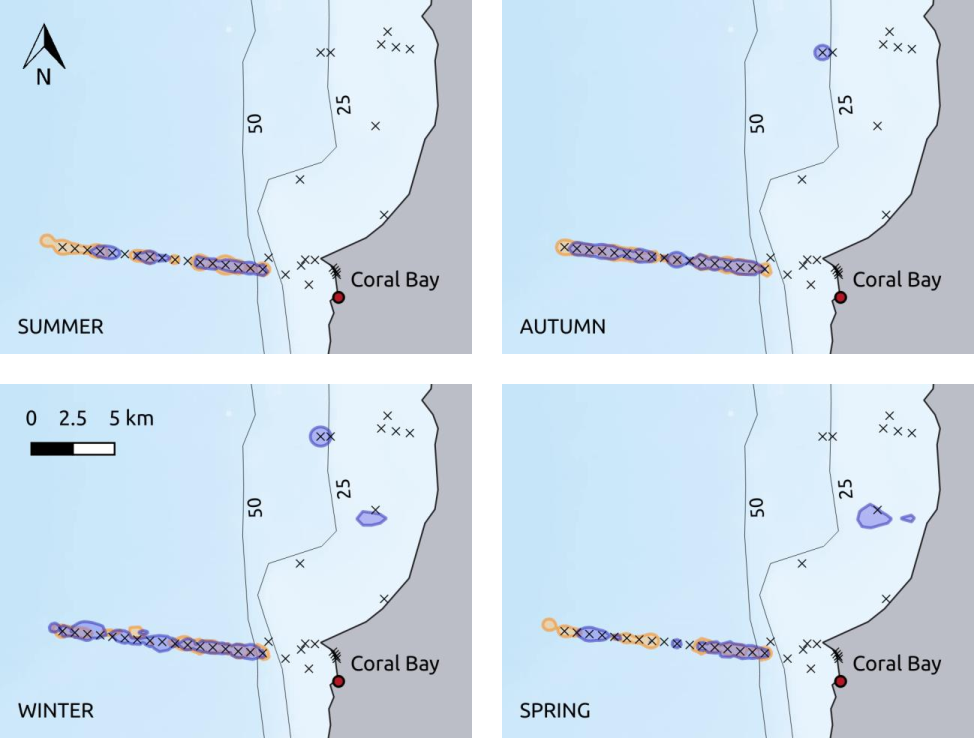
\includegraphics[width=0.9\textwidth]{../Results/Coral_bay.pdf}
		\caption{Seasonal variation in core kernel utilisation areas of \textit{Carcharhinus obscurus} (purple) and \textit{Carcharhinus plumbeus} (orange), within the Stanley Pool and southern line arrays, Ningaloo reef, WA. Black crosses show acoustic receiver locations and water depth is given parallel to each bathymetry contour This map was generated using QGIS \citep{QGISDevelopmentTeam2019}, with a base map shapefile \citep{AustralianBureauofStatistics2011}, bathymetric contour shapefile \citep{GEBCOCompilationGroup2019} and bathymetry raster \citep{Whiteway2009}.}
		\label{depth_south}
	\end{figure}		
		
	\newpage
	\section{Discussion}
	
	This study aimed to address the drivers of residential movements and whether they could be used to predict large scale movements by comparing variation in acoustic network use, area and depth use and residency between and within species. This was examined using acoustic telemetry data on two species of shark dusky, \textit{Carcharhinus obscurus}, and sandbar, \textit{Carcharhinus plumbeus}.

	\subsection{Network Use}
	
	Spatial network analysis was used to assess use of the reef. Network density was chosen as the best network metric for this system as it contained line arrays as opposed to conventional grid arrays, and spanned a much larger area, rendering any network metric reliant on equal spacing of nodes meaningless. Network density is not as dependent on this, as it gives a proportion of the edges used out of the total possible edges, as opposed to the length of each edge.\\
	\\
	Network density showed very little variance between species, indicating both species use similar proportions of the reef. When split by season, dusky sharks showed a distinct pattern, with proportion used decreasing significantly in winter then increasing again in the summer. 
	
	
	Males = larger network than females in C. amblyrhynchos - grey reef shark - \citep{Espinoza2015}
	no change in network size with sex in bull and silvertip - \citep{Espinoza2015}
	Highlu variable between individuals = \citep{Lea2016}
	increased activity at night in several adult shark species but no evidence in juveniles - sixgill, leopard, white tip reef, grey reef and lemon \citep{Speed2010}
	
	The close proximity of receivers within the same line array could have increased probability of detection however receivers in the same line were at different depths, removing a proportion of this bias, however outputs should still be interpreted with reference to other metrics;
	- justification of network density	
	- results of network models and interpretations - ecologically
	- individual variation in networks 

	
	\subsection{Area \& Depth Use}
	
	- KUD results and implications
	main factor in grey reef and bull sharks = size \citep{Speed2010} which is not application for this study due to small size range
	- individual variation in KUD
	
	- Depth analysis through detection data and implications

	
	- seasonal - 
	During gestation female sand tiger sharks C. taurus, move north into warmer waters - link with moving to shallower water - could be gestation - and also carry out large scale migrations in S Africa and give birth in cooler southern waters \citep{Dicken2007}
	juv sandbars = deeper dives in winter than summer - E coast of N america \citep{Speed2010}
	juv lemon sharks - temp for optimal metabolic performance - movements over time with climate change/ drives depth changes over seasons \citep{Speed2010}
	- time of day - 
	links to movements of prey - in Caribbean reef shark more time spent at surface at night due to prey movements up \citep{Speed2010}
	
	
	- individual variation in depths

	

	\subsection{Residency \& Migration}
	
	- results from RI models and ecological implications
	
	resident in ningaloo due to high productivity of coral reefs \citep{Espinoza2016}
	females more likely in bull shark more likely to leave residential area than males - for giving birth \citep{Espinoza2016} - in contrast to dusky where the majority of males were migratory
	
	- individual variation in RI
	
	partial migration in bull sharks - ind variation - not all mature females migrate, some remain resident in E Aus \citep{Espinoza2016} - could be why some duskies remain
	partial also seen in Port Jackson sharks, E Aus - \citep{Bass2017}
	partial to most likely five birth in tiger sharks in Hawaii but not all mature females and mainly females \citep{Papastamatiou2013}
	
	- lack of correlation with migration status in duskies - ecological applications
	
	very little difference in sex distribution = fisheries captures in 1994-1999 in south gave very even dis of both species of both sexes caught \citep{McAuley2003}
	
	- drivers of residential movements
	
	cooler water temp in S Africa = upwellings along coast = > nutrients and increased teleosts so more predators present incl sandbars \citep{Wintner2018}
	very little effect of water temperature on dusky movements in S Africa - could be more resilient hence detections further south than sandbars
	in tiger sharks, movements between reefs are suggested to be due to foraging in Hawaii and individual based \citep{Papastamatiou2013}
	
	- prediction of migration
	
	very little effect of water temperature on dusky movements in S Africa - could be more resilient hence detections further south than sandbars \citep{Wintner2018}
	seasonal environ change, reprod and foraging \citep{Espinoza2015}
	give birth - e.g. move into temperate waters seen in C taurus though warmer for gestation \citep{Dicken2007}
	segregated by age - sandbar observed in more temperature waters when young - in south at depths \textgreater 80m, neonates from Geraldton to Broome and caught in south below 26S \citep{McAuley2005} - extent of range potentially not as far south as perth receivers - issue with layout of receivers
	but not being picked up on receivers in South - narrow continental shelf along south coast in comparison with Ningaloo - may not be picked up - also adults tagged in south
	sandbar catch much lower between 1994 and 1999 than dusky but were present in south \citep{McAuley2003}
	isolated reefs more likely to remain resident than well connected \citep{Espinoza2015} - Ningaloo not isolated so more likely to migrate
	sandbars physiologically in heat at same time movement occurs within duskies \citep{McAuley2005}
	
		
		
	
	- eval. of Acoustic Telemetry
	only gives presence or absence data but valuable long term \citep{Bass2017}
	relatively inexpensive \citep{Speed2010}
	increased understanding of marine predators \citep{Espinoza2016}
	HUGE GAP in middle of arrays

	- future directions for research
	
	combination of catch data, such as that used in \citep{Braccini2017a} with acoustic data and more receivers in central range or deeper southern range to accurately assess risk
	look further into depth use - receivers at greater range of depths as space use may change with climate change - higher temp = nearer shore, effects of climate change on this largely unquantified so far \citep{Speed2010}
	evidence of size being important - larger networks \citep{Espinoza2015}and greater distances moved (Papamatadiou 2013) - wider size range of sharks

	\subsection{Conclusions}
	
	As species that are slow to mature and have a low fecundity \citep{Cortes2000}, dusky and sandbar sharks are both slow to recover from overexploitation \citep{Rogers2013}. 
	
	management has been well implemented - easier than east coast due to single jurisdiction of WA. \citep{Heupel2015}

	- high individual variability
	challenging to explain \citep{Espinoza2015}
	- seasonality
	- lack of sexual influence
	- overall drivers of residential movements
	- can we predict large scale movements
	
	\newpage
	
	\noindent{\large \textit{Acknowledgements}}\\
	
	\noindent{\large \textit{Data \& Code Availability}}\\
	\\
	All R code and raw data files are available in my GitHub repository as well as a bash script detailing the order to run each script file: https://github.com/KBicks/CMEECourseWork/tree/master/Project.  
	
	\newpage
	
	\section{References}
	
	\bibliography{Bickerton_Katherine_CMEEMRes_2019}
	
	\newpage
	
	
	\section{Appendices}
	
	\setcounter{table}{0}
	\renewcommand{\thetable}{A\arabic{table}}
	
	\subsection{Model Outputs}
	
	
	\begin{table}[h!]
		\caption{GLMM outputs for network density models, using a log normal distribution. All models used individual ID as a random effect and fixed effects are given in the first column. The null model is given by network density $\sim$ 1, and was used as a comparison to calculate $\chi^2$ and p-values for other models. Rows are divided into sections for both species (all, n = 111), dusky sharks (\textit{C. obscurus}, n = 52) \& sandbar sharks (\textit{C. plumbeus}, n = 58). Metrics of fit used are Akaike Information Criterion (AIC), $R^2$ marginal giving the variance explained by fixed effects, and $R^2$ conditional giving the variance explained by the whole model, the output of the likelihood ratio test, $\chi^2$ and p-value, and the degrees of freedom (df). Bold text indicates the best fitting model and significant metrics. Models with multiple fixed variable were also tested however single variable models had better fit.}
		\centering
		\begin{tabular}{@{}lcccccc@{}}
			& \textit{AIC} & {$R^2_m$} & {$R^2_c$} & {$\chi^2$} & \textit{df} & \textit{p}      \\ 
			\midrule
			\textit{All}                           &              &              &              &               &             &                 \\
			Network Density $\sim$ 1 & 66.01 & -  & 0.748 & - & 3 & - \\
			Network Density $\sim$ Species          & 65.60        & 0.047        & 0.752        & 2.514         & 4           & 0.113           \\
			Network Density $\sim$ Sex              & 67.52        & 0.049        & 0.755        & 2.692         & 4           & 0.101           \\
			\textbf{Network Density $\sim$ Season}           & \textbf{65.09}        & 0.032        & 0.763        & 12.47         & 6           & 0.006           \\
			Network Density $\sim$ Time of Day      & 67.05        & 0.010        & 0.908        & 7.862         & 4           & 0.005           \\ \midrule
			\textit{Carcharhinus obscurus}         &              &              &              &               &             &                 \\
			Network Density $\sim$ 1 & 59.45 & -  & 0.779 & - & 2 & - \\
			Network Density $\sim$ Sex              & 59.95        & 0.130        & 0.785        & 3.436         & 4           & 0.064           \\
			\textbf{Network Density $\sim$ Season}           & \textbf{48.39}        & \textbf{0.159}        & 0.850        & 20.28         & 6           & \textbf{\textless 0.001} \\
			Network Density $\sim$ Time of Day      & 58.66        & 0.021        & 0.933        & 10.26         & 4           & 0.0013          \\
			Network Density $\sim$ Migratory Status & 60.47        & 0.034        & 0.778        & 0.738         & 4           & 0.390           \\ \midrule
			\textit{Carcharhinus plumbeus}         &              &              &              &               &             &                 \\
			Network Density $\sim$ 1 & 7.460 & -  & 0.709 & - & 3 & - \\
			Network Density $\sim$ Sex              & 9.420        & 0.012        & 0.712        & 0.334         & 4           & 0.563           \\
			\textbf{Network Density $\sim$ Season}           & \textbf{5.115}        & 0.033        & 0.733        & 8.172         & 6           & 0.042           \\
			Network Density $\sim$ Time of Day      & 8.456        & 0.005        & 0.870        & 1.295         & 4           & 0.255           \\ \bottomrule
		\end{tabular}
		\label{network_outputs}
	\end{table}
	
	\newpage
	
	\begin{table}[h!]
		\caption{GLMM outputs for kernel density utilisation models (KUD), using a gamma distribution. All models used individual ID as a random effect and fixed effects are given in the first column. The null model is given by KUD $\sim$ 1, and was used as a comparison to calculate $\chi^2$ and p-values for other models. Rows are divided into sections for both species (all, n = 77), dusky sharks (\textit{C. obscurus}, n = 39) \& sandbar sharks (\textit{C. plumbeus}, n = 39). Metrics of fit used are Akaike Information Criterion (AIC), the output of the likelihood ratio test, $\chi^2$ and p-value, and the degrees of freedom (df). Two types of AIC are used as sample size was too small to subset both season and time of day, giving two subsets with non comparable AIC values (se = seasonal subset and dn = time of day subset). Bold text indicates the best fitting model and significant metrics. Models with multiple fixed variable were also tested however single variable models had better fit.}
		\centering
		\begin{tabular}{@{}lccccc@{}}
			& $AIC_{se}$ & $AIC_{dn}$ & $\chi^2$  & \textit{df} & \textit{p}               \\ \midrule
			\textit{All}                   &       &       &       &    &                 \\
			KUD $\sim$1                    & 345.0 & 288.3 & -     & 3  & -               \\
			\textbf{KUD $\sim$Species}              & \textbf{334.9} & \textbf{285.8} & 12.13 & 4  & \textbf{\textless 0.001} \\
			KUD $\sim$Sex                  & 346.5 & 289.8 & 0.584 & 4  & 0.445           \\
			KUD $\sim$Season               & 347.3 & -     & 3.702 & 6  & 0.230           \\
			KUD $\sim$Time of Day          & -     & 289.8 & 0.476 & 4  & 0.491           \\ \midrule
			\textit{Carcharhinus obscurus} &       &       &       &    &                 \\
			KUD $\sim$1                    & \textbf{178.2} & 163.1 & -     & 3  & -               \\
			\textbf{KUD $\sim$Sex}                  & \textbf{178.2} & \textbf{162.2} & 2.032 & 4  & 0.154           \\
			KUD $\sim$Season               & 181.8 & -     & 2.485 & 6  & 0.478           \\
			KUD $\sim$Time of Day          & -     & 165.1 & 0.089 & 4  & 0.765           \\
			KUD $\sim$Migratory Status     & 179.5 & 164.1 & 0.703 & 4  & 0.402           \\ \midrule
			\textit{Carcharhinus plumbeus} &       &       &       &    &                 \\
			KUD $\sim$1                    & \textbf{153.4} & 124.1 & -     & 3  & -               \\
			KUD $\sim$Sex                  & 155.4 & 126.1 & 0.007 & 4  & 0.935           \\
			KUD $\sim$Season               & 158.3 & -     & 1.020 & 6  & 0.796           \\
			\textbf{KUD $\sim$Time of Day}          & -     & \textbf{123.6} & 2.52  & 4  & 0.112           \\ \bottomrule
		\end{tabular}
		\label{KUD_outputs}
	\end{table}
	
	
	
	\newpage
	
	
	\begin{table}[h!]
		\caption{GLMM outputs for residency index models (RI), using a log normal distribution. All models used individual ID as a random effect and fixed effects are given in the first column. The null model is given by RI $\sim$ 1, and was used as a comparison to calculate $\chi^2$ and p-values for other models. Rows are divided into sections for both species (all, n = 110), dusky sharks (\textit{C. obscurus}, n = 49) \& sandbar sharks (\textit{C. plumbeus}, n = 59). Metrics of fit used are Akaike Information Criterion (AIC), $R^2$ marginal giving the variance explained by fixed effects, and $R^2$ conditional giving the variance explained by the whole model, the output of the likelihood ratio test, $\chi^2$ and p-value, and the degrees of freedom (df). Two types of AIC are used as sample size was too small to subset both season and time of day, giving two subsets with non comparable AIC values (se = seasonal subset and dn = time of day subset). Bold text indicates the best fitting model and significant metrics. Models with multiple fixed variable were also tested however single variable models had better fit.}
		\centering
		\begin{tabular}{lccccccc}
			& $AIC_{se}$ & $AIC_{dn}$ & $R^2_m$ & $R^2_c$ & $\chi^2$ & \textit{df} & \textit{p}      \\ \hline
			\textit{All}                   &             &             &                         &                         &                        &             &                 \\
			RI $\sim$ 1                     & -646.3      & -1076.0     & -                       & 0.992                   & -                      & 3           & -               \\
			RI $\sim$ Species               & -345.8      & -1075.7     & 0.038                   & 0.992                   & 1.422                  & 4           & 0.233           \\
			RI $\sim$ Sex                   & -644.9      & -1074.4     & 0.018                   & 0.992                   & 0.605                  & 4           & 0.437           \\
			\textbf{RI $\sim$ Season     }           & \textbf{-730.7}      & -           & 0.037                   & 0.994                   & 90.38                  & 6           & \textbf{\textless 0.001 }\\
			\textbf{RI $\sim$ Time of Day}           & -           & \textbf{-1217.6}     & 0.006                   & 0.999                   & 143.6                  & 4           & \textbf{\textless 0.001} \\
			\hline
			\textit{Carcharhinus obscurus} &             &             &                         &                         &                        &             &                 \\
			RI $\sim$ 1                     & -404.8      & -610.0      & -                       & 0.996                   & -                      & 3           & -               \\
			RI $\sim$ Sex                   & -406.0      & -608.3      & \textbf{0.182}                   & 0.996                   & 2.155                  & 4           & 0.142           \\
			\textbf{RI $\sim$ Season}                & \textbf{-461.8}      & -           & \textbf{0.222}                   & 0.998                   & 63.00                  & 6           & \textbf{\textless 0.001 }\\
			RI $\sim$ Time of Day           & -           & \textbf{-740.5}      & 0.050                   & 0.999                   & 132.5                  & 4           & \textbf{\textless 0.001} \\
			RI $\sim$ Migratory Status      & -403.7      & -734.9      & 0.060                   & 0.996                   & 0.921                  & 4           & 0.337           \\
			\hline
			\textit{Carcharhinus plumbeus} &             &             &                         &                         &                        &             &                 \\
			RI $\sim$ 1                     & -299.1      & -509.8      & -                       & 0.989                   & -                      & 3           & -               \\
			RI $\sim$ Sex                   & -297.4      & -507.9      & 0.015                   & 0.989                   & 0.288                  & 4           & 0.592           \\
			\textbf{RI $\sim$ Season}                & \textbf{-349.0}      & -           & 0.033                   & 0.991                   & 55.92                  & 6           & \textbf{\textless 0.001} \\
			RI $\sim$ Time of Day           & -           & \textbf{-589.1}      & 0.004                   & 0.999                   & 81.29                  & 4           & \textbf{\textless 0.001} \\
			\hline
		\end{tabular}
		\label{ri_outputs}
	\end{table}
	
	\newpage
	
	\begin{table}[h!]
		\caption{GLMM outputs for daily detection models (RI), using a log normal distribution. All models used individual ID as a random effect and fixed effects are given in the first column. The null model is given by number of detections $\sim$ 1, and was used as a comparison to calculate $\chi^2$ and p-values for other models. Rows are divided into sections for both species (all, n = 100), dusky sharks (\textit{C. obscurus}, n = 30) \& sandbar sharks (\textit{C. plumbeus}, n = 40). Metrics of fit used are Akaike Information Criterion (AIC), $R^2$ marginal giving the variance explained by fixed effects, and $R^2$ conditional giving the variance explained by the whole model, the output of the likelihood ratio test, $\chi^2$ and p-value, and the degrees of freedom (df). Two types of AIC are used as sample size was too small to subset both season and time of day, giving two subsets with non comparable AIC values (se = seasonal subset and dn = time of day subset). Bold text indicates the best fitting model and significant metrics. Models with multiple fixed variable were also tested however single variable models had better fit.}
		\centering
		\begin{tabular}{lccccccc}
			& $AIC_{se}$ & $AIC_{dn}$ & $R^2_m$ & $R^2_c$ & $\chi^2$ & \textit{df} & \textit{p}      \\ \hline
			\textit{All}                   &             &             &                         &                         &                        &             &                 \\
			Det $\sim$1                    & 101930      & 124948      & -                       & 0.221                   & -                      & 3           & -               \\
			Det $\sim$Species              & 101932      & 124949      & \textless 0.001         & 0.220                   & 0.180                  & 4           & 0.671           \\
			Det $\sim$Sex                  & 101930      & 124947      & \textless 0.001         & 0.216                   & 2.083                  & 4           & 0.149           \\
			\textbf{Det $\sim$Season}               & \textbf{101232}      & -           & \textless 0.001         & 0.234                   & 260.4                  & 7           & \textless 0.001 \\
			Det $\sim$Time of Day          & -           & 124915      & \textless 0.001         & 0.155                   & 34.72                  & 4           & \textbf{\textless 0.001} \\
			Det $\sim$Depth Band           & 101477      & 124549      & \textless 0.001         & 0.233                   & 463.4                  & 8           & \textbf{\textless 0.001} \\ \hline
			\textit{Carcharhinus obscurus} &             &             &                         &                         &                        &             &                 \\
			Det $\sim$1                    & 7406.3      & 7895.9      & -                       & 0.140                   & -                      & 3           & -               \\
			Det $\sim$Sex                  & 7407.5      & 7897.1      & \textless 0.001         & 0.137                   & 0.813                  & 4           & 0.367           \\
			Det $\sim$Season               & 7399.0      & -           & \textless 0.001         & 0.152                   & 13.30                  & 6           & 0.004           \\
			Det $\sim$Time of Day          & -           & 7890.1      & \textless 0.001         & 0.120                   & 7.861                  & 4           & 0.005           \\
			Det $\sim$Migratory Status     & 7408.0      & 7897.4      & \textless 0.001         & 0.139                   & 0.276                  & 4           & 0.600           \\
			\textbf{Det $\sim$Depth Band}           & \textbf{7354.9}      & 7846.9      & 0.0012                  & 0.136                   & 59.35                  & 7           & \textbf{\textless 0.001} \\ \hline
			\textit{Carcharhinus plumbeus} &             &             &                         &                         &                        &             &                 \\
			Det $\sim$1                    & 93174       & 116707      & -                       & 0.231                   & -                      & 3           & -               \\
			Det $\sim$Sex                  & 93174       & 116707      & \textless 0.001         & 0.224                   & 1.365                  & 4           & 0.243           \\
			\textbf{Det $\sim$Season}               & \textbf{92927}       & -           & \textless 0.001         & 0.244                   & 252.6                  & 6           & \textbf{\textless 0.001} \\
			Det $\sim$Time of Day          & -           & 116678      & \textless 0.001         & 0.177                   & 31.26                  & 4           & \textbf{\textless 0.001} \\
			\textbf{Det $\sim$Depth Band}           & 92733       & \textbf{116303}      & \textless 0.001         & 0.235                   & 450.8                  & 8           & \textbf{\textless 0.001} \\ \hline
		\end{tabular}
		\label{det_outputs}
	\end{table}
	
	
\end{document}